\documentclass[aspectratio=169,12pt]{beamer}
\usefonttheme{serif}
\useinnertheme{default}
\useoutertheme{default}
\setbeamertemplate{navigation symbols}{}
\setbeamertemplate{footline}[frame number]

\usepackage[utf8]{inputenc}
\usepackage[T1]{fontenc}
\usepackage{lmodern}
\usepackage{tikz}
\usetikzlibrary{arrows.meta,positioning,calc,fit}
\usepackage{amsmath}
\usepackage{ragged2e}
\usepackage{multicol}

\definecolor{wikiblue}{RGB}{51,102,204}
\definecolor{wikidark}{RGB}{32,33,34}
\definecolor{wikigray}{RGB}{84,89,93}
\definecolor{wikiborder}{RGB}{200,204,209}
\definecolor{wikibox}{RGB}{248,249,250}
\definecolor{wikibox2}{RGB}{234,236,240}
\definecolor{wikilightblue}{RGB}{238,243,255}
\definecolor{wine}{RGB}{114,47,55}

\setbeamercolor{normal text}{fg=wikidark,bg=white}
\setbeamercolor{title}{fg=wikidark}
\setbeamercolor{frametitle}{fg=wikidark,bg=white}
\setbeamercolor{structure}{fg=wikiblue}
\setbeamercolor{block title}{fg=wikidark,bg=wikibox2}
\setbeamercolor{block body}{fg=wikidark,bg=wikibox}
\setbeamercolor{alertblock title}{fg=wikidark,bg=wikibox2}
\setbeamercolor{alertblock body}{fg=wikidark,bg=wikibox}
\setbeamerfont{frametitle}{size=\large}
\setbeamerfont{block title}{size=\normalsize}
\setbeamertemplate{blocks}[rounded][shadow=false]

\tikzset{
  wikiarrow/.style={->, thick, draw=wikigray, >=Latex},
  wikistep/.style={
    draw=wikiborder,
    fill=wikibox,
    rounded corners=1.5pt,
    thick,
    align=center,
    text=wikidark,
    font=\scriptsize,
    minimum width=3.25cm,
    minimum height=0.82cm,
    inner sep=2.5pt
  },
  wikistephi/.style={
    draw=wikiborder,
    fill=wikilightblue,
    rounded corners=1.5pt,
    thick,
    align=center,
    text=wikidark,
    font=\scriptsize,
    minimum width=3.25cm,
    minimum height=0.82cm,
    inner sep=2.5pt
  },
  wikiboxnote/.style={
    draw=wikiborder,
    fill=wikibox,
    rounded corners=1.5pt,
    thick,
    align=left,
    text=wikidark,
    font=\scriptsize,
    inner sep=4pt,
    text width=4.15cm
  }
}

\begin{document}

%--- Slide 1 ---
\begin{frame}[t]{Article Generation Pipeline}
\hspace*{-0.035\textwidth}%
\begin{minipage}{1.07\textwidth}
\begin{columns}[T,totalwidth=\linewidth,onlytextwidth]
\column{0.55\linewidth}
\centering
\resizebox{\linewidth}{!}{%
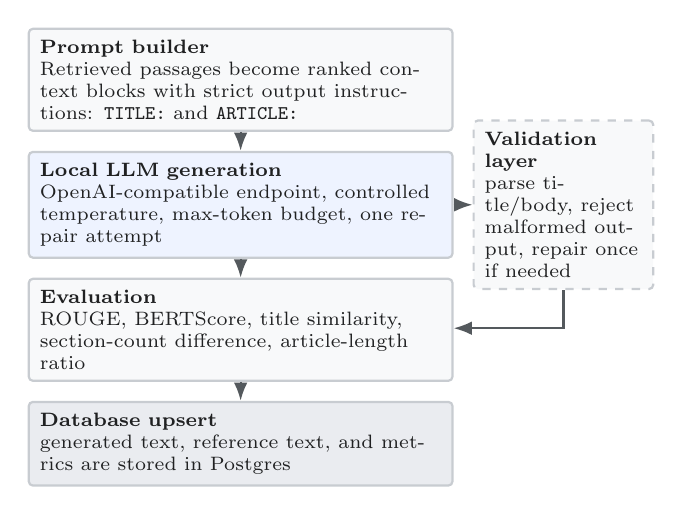
\begin{tikzpicture}[node distance=0.24cm]
  \node[wikiboxnote, text width=5.1cm] (p) {\textbf{Prompt builder}\\Retrieved passages become ranked context blocks with strict output instructions: \texttt{TITLE:} and \texttt{ARTICLE:}};
  \node[wikiboxnote, fill=wikilightblue, text width=5.1cm, below=of p] (g) {\textbf{Local LLM generation}\\OpenAI-compatible endpoint, controlled temperature, max-token budget, one repair attempt};
  \node[wikiboxnote, text width=5.1cm, below=of g] (e) {\textbf{Evaluation}\\ROUGE, BERTScore, title similarity, section-count difference, article-length ratio};
  \node[wikiboxnote, fill=wikibox2, text width=5.1cm, below=of e] (d) {\textbf{Database upsert}\\generated text, reference text, and metrics are stored in Postgres};
  \node[wikiboxnote, dashed, text width=2.0cm, right=0.24cm of g] (v) {\textbf{Validation layer}\\parse title/body, reject malformed output, repair once if needed};

  \draw[wikiarrow] (p) -- (g);
  \draw[wikiarrow] (g) -- (e);
  \draw[wikiarrow] (e) -- (d);
  \draw[wikiarrow] (g.east) -- (v.west);
  \draw[wikiarrow] (v.south) |- ($(e.east)+(0,0.02)$);
\end{tikzpicture}%
}
\column{0.42\linewidth}
\vspace*{-0.8cm}

\begin{block}{Runner behavior}
\scriptsize
\begin{itemize}
  \item single-article or batch execution
  \item schema creation for \texttt{generated\_articles}
  \item skip-existing logic from database state
  \item per-article error isolation for long runs
\end{itemize}
\end{block}

\vspace{0.04cm}
\begin{block}{Cost profile}
\scriptsize
Generation dominates runtime. Retrieval, prompt assembly, and database writes are much cheaper, while larger $k$ (the number of retrieved passages included in the prompt) and larger token budgets mainly increase latency.
\end{block}

\vspace{0.04cm}
\begin{block}{LLM used (With Ollama)}
\scriptsize
Started with gemma-2-2b, then went with Phi-3.5-mini-instruct for 16K context window.
\end{block}
\end{columns}
\end{minipage}
\end{frame}

%--- Slide 2 ---

\begin{frame}[t]{The Prompt}
\vspace{-0.50cm}

{\color{wine}\ttfamily\scriptsize\RaggedRight\sloppy
\begin{multicols}{3}
Write a neutral encyclopedia-style article in plain text using only the supplied passages.\par
Use only supported facts from the passages. Do not invent details.\par
If a detail is uncertain, conflicting, or weakly supported, leave it out.\par
Do not mention passages, retrieval, scores, evidence, or source metadata.\par
Do not write commentary, advice, analysis notes, a Q\&A answer, or a summary about the evidence.\par
Do not address the reader.\par
Do not write like a review, recommendation, or box-office report.\par
Do not output tables, lists, charts, headings, markdown, or code fences.\par
Write continuous prose paragraphs only.\par
Prefer broad coverage of the most important facts over over-expanding one aspect.\par
Avoid repeating the same fact in different wording.\par
Higher relevance passages matter more than lower relevance passages.\par
Use lower-scoring passages only for extra detail, not to override stronger evidence.\par
If supported by the passages, cover subject, background, production or development, release, reception, and performance.\par
If an aspect is not supported, omit it.\par
This article has \textit{\color{black}\{bundle.available\_passage\_count\}} indexed passages in total.\par
The prompt contains \textit{\color{black}\{len(passages)\}} selected passages.\par
Aim for about \textit{\color{black}\{target\_words\}} words and about \textit{\color{black}\{target\_paragraphs\}} paragraphs.\par
The title must be exactly the target title.\par
The first line must be exactly: TITLE: <article title>\par
Then a blank line.\par
Then a line that is exactly: ARTICLE:\par
Then the article body in plain prose paragraphs.\par
\small\textbf{If you cannot follow this exact format, output nothing.}
\end{multicols}
}
\end{frame}
%--- Slide 3 ---
\begin{frame}[t]{Conclusion \& Future Work}
\vspace{-0.10cm}
\hspace*{-0.025\textwidth}%
\begin{minipage}{1.05\textwidth}
\begin{block}{Conclusion}
\scriptsize
\justifying
With this approach it is possible -- with reasonable accuracy -- to reconstruct a Wikipeda article just from its citations.
\end{block}

\vspace{0.08cm}
\begin{columns}[T,totalwidth=\linewidth,onlytextwidth]
\column{0.47\linewidth}
\begin{block}{Weaknesses}
\scriptsize
\begin{itemize}
  \item A majority of citations is unavailable, mostly through some kind of paywalls. There were also cases of webcrawler blocks.
  \item Runtimes are absurdly long for consumer hardware.
  \item Article generation often aborts or is much too short.
\end{itemize}
\end{block}

\column{0.47\linewidth}
\begin{block}{Strengths}
\scriptsize
\begin{itemize}
  \item Topic inference works surprisingly well.
  \item Easily expandable. We have a robust foundation, and were always limited by time, never by ideas.
\end{itemize}
\end{block}
\end{columns}

\vspace{0.04cm}
\begin{alertblock}{Future Work}
\scriptsize
Strong evaluation gains are expected from a better retrieval structure and more controlled generation rather than from rebuilding the pipeline itself.
\end{alertblock}

\end{minipage}
\end{frame}

\end{document}
